\title{Appendices}

\documentclass[12pt]{article}
\usepackage{amsmath}
\usepackage{mathabx}
\usepackage{graphics}
\usepackage[top=0.75in, bottom=0.75in, left=1in, right=1in]{geometry}
\usepackage{tabu}
\usepackage[english]{babel}
\usepackage{natbib}
\bibliographystyle{evolution}
\usepackage{rotating}
\usepackage[capitalize, sort&compress]{cleveref}
\usepackage{float}
%\newcommand{\crefrangeconjunction}{--}
%\crefname{section}{Sect.}{Sects.}
%\crefname{equation}{Eq.}{Eqs.}
%\crefformat{equation}{Eq.~#2#1#3}
%\crefrangeformat{equation}{Eqs.~#3#1#4--#5#2#6}
%\crefmultiformat{equation}{Eqs.~#2#1#3}{--#2#1#3}{, #2#1#3}{ and~#2#1#3}

% for comments visible in the compiled pdf
%\usepackage{color}
%\definecolor{orange}{rgb}{0.8,0.4,0}
%\newcommand{\eeg}[1]{{\em \color{orange} #1}}

% Tell latex how it can introduce linebreaks if necessary.
\hyphenation{Bar-thol-o-mew}

\date{\vspace{-5ex}}

\begin{document}
\maketitle

Change in temperature...

\section{Zenith angle and time of sunrise}
We use the same equation as in \citet{Campbell2012} to model zenith angle ($\psi$) as a function of the time of the day $t$ and latitude $\phi$.
We have
\begin{equation}  \label{eq:psi}
\cos(\psi) = \sin(\phi) \sin(\delta) + \cos(\phi) \cos(\delta) \cos[15 (t- t_0)],
\end{equation}
where $\delta$ represents solar declination which varies between 23.45$^\circ$ and  -23.45$^\circ$ between summer and winter solstice, respectively ($\delta$ is given by equation 11.2 in \citet{Campbell2012} and only depends of the day of the year).
$t_0$ represents the time of solar noon and varies with longitude but since we are interested in latitudinal variation, we fix $t_0 = 12$.

At any given latitude $\phi$ and day of the year---in the expression of $\delta$---the time of sunrise $t_{rise}$ is the solution of the next equation in the time interval $[0,12]$ when $\psi = 0$

\begin{equation}
t_{rise} =  \frac{1}{15} \left( t_0 +  \arccos \left[ \frac{\cos(\psi = 0) - \sin(\phi) \sin(\delta)}{\cos(\phi) \cos(\delta)} \right] \right).
\end{equation}


%\begin{figure}
%\begin{center}
%	\scalebox{0.75}{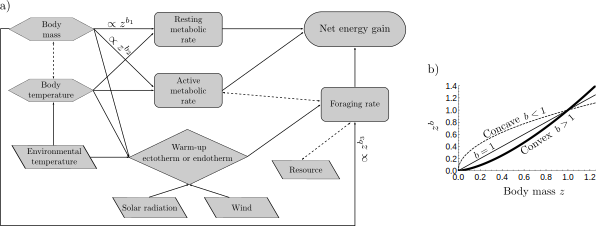
\includegraphics{fig1}}
%	\caption{Change in solar radiation during the course of the day at different latitudes---color coded and labeled numbers.
%	Northern latitudes are denoted by positive numbers.
%	}
%	\label{fig:rad}
%\end{center}
%\end{figure}

\section{Geometric property of the body}
For simplicity we assume that the individual is shaped as a the half of sphere (\cref{fig:geo}, such approximation can be valid for insects such as dung beetles).
Considering a sphere is practical as we only have one free variable:  the radius $r$.
\begin{figure}
\begin{center}
	\scalebox{0.5}{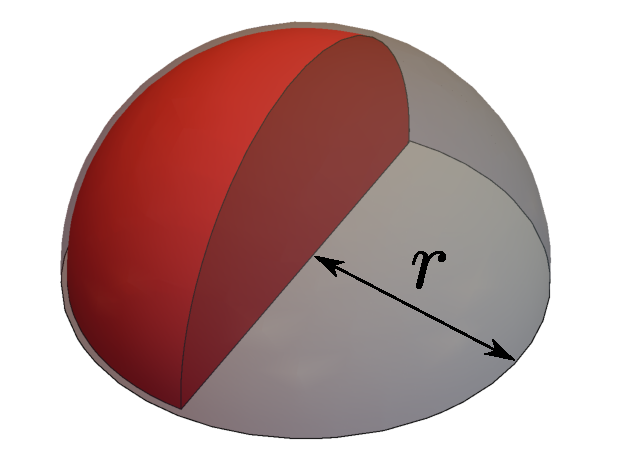
\includegraphics{body_vita}}
	\caption{Geometric representation of the shape of an individual.
	The thorax is in red and the non-thorax in gray.
	For clarity, we shrank the thorax but the radius is the same as the radius of the non-thorax.
	}
	\label{fig:geo}
\end{center}
\end{figure}
The volume of half a sphere is $V = \frac{2}{3} \pi r^3$ and the surface $A = \pi r^2 + 2 \pi r^ 2 = 3 \pi r^2$ (the first term of the summation represents the surface at the bottom and the second the cap).
We assume that the thorax occupies half of the body with volume $V_{th} = V/2$ and surface $A_{th} = \pi r^2 + \pi r^2 = 2 \pi r^2$ (the second term is half of the cap whereas the first is the same as the surface of the bottom just folded upward).

Knowing body mass $z$ and density $d$, we can convert mass into volume $ V = z/d$.
The radius $r = \left( \frac{3V}{2 \pi} \right)^{1/3}$

\section{Derivation of  equation 8 in the main text}
In this section, we derive sufficient conditions where net energy gain peaks at intermediate body size given foraging time is limited.
We defined net energy gain by:
\begin{equation} \label{eq:main}
	E_n(z, \tau_f) = E_g(z,\tau_f) - E_d(z, \tau_f).
\end{equation}
The energetic gain is
\[
	E_g(z,\tau_f - \tau_w) = (\tau_f - \tau_w) e_g(z),
\]
with
\begin{equation} \label{eq:eg}
	e_g(z) = a_3 z^{b_3} \times \rho  = g(z) \times \rho.
\end{equation}
%
The energetic cost is
\begin{equation} \label{eq:ed}
	E_d(z, \tau_f) = \int_0^{t_i} e_b(z, t) dt + \int_{t_i + \tau_w}^{t_i + \tau_f } e_a(z,t) dt + \int_{t_i+\tau_f}^{24} e_b(z, t) dt
\end{equation}
where,
\begin{equation} \label{eq:eb}
	e_b(z, t) = a_1 z^{b_1} e^{-E/[k (T_b(t)+ 273.15)]} =  a_1 z^{b_1} \theta_1
\end{equation}
and
\begin{equation} \label{eq:ea}
	e_a(z,t) = a_2 z^{b_2}  e^{-E/[k (\max(T_w(z_{th}), T_e(t))+ 273.15)]} =  a_2 z^{b_2} \theta_2.
\end{equation}

For simplicity, we assume that there is no warm-up and temperature is constant during the day so that $\theta_1$ and $\theta_2$ do not depend on time.
We want to derive a relationship where \cref{eq:main} becomes a non-monotonic function of body mass $z$.
Two conditions are  necessary: net energy gain should be positive and the derivative of the net energy gain should change sign from positive to negative.
By definition,
\begin{flalign*}
	E_n(z,\tau_f) & = e_g(z) \times \tau_f  - \left( e_a(z) \times \tau_f + e_b(z) \times (24 - \tau_f ) \right) \\
			&  = \rho a_3 z^{b_3} \times \tau_f  - \left( a_2 z^{b_2}  \theta_2 \times \tau_f +  a_1 z^{b_1} \theta_1 \times ( 24 -\tau_f) \right)
\end{flalign*}
After simple algebraic manipulation, $E_n$ is positive if and only if
\begin{equation}\label{ineq:1}
	\rho > c_1 z^ {b_1 - b_3}  \tfrac{24 - \tau_f}{\tau_f}  + c_2  z^ {b_2 - b_3},
\end{equation}
where $c_1 = \dfrac{a_1}{a_3} \theta_1$ and $c_2 = \dfrac{a_2}{a_3} \theta_2$.
%
For the second condition, the derivative is
\begin{flalign*}
	\frac{d}{dz} E_n(z,\tau_f) & = \rho a_3  b_3 z^{b_3 - 1} \times \tau_f  - \left( a_2 b_2 z^{b_2 -1 }  \theta_2 \times \tau_f +  a_1  b_1 z^{b_1- 1} \theta_1 \times ( 24 -\tau_f) \right),
\end{flalign*}
and is negative if and only if
\begin{equation}\label{ineq:2}
	\rho < c'_1 z^ {b_1 - b_3}  \tfrac{24 - \tau_f}{\tau_f}  + c'_2  z^ {b_2 - b_3},
\end{equation}
where $c'_1 = \dfrac{a_1 b_1}{a_3 b_3} \theta_1$ and $c'_2 = \dfrac{a_2 b_2}{a_3 b_3} \theta_2$.
Thus a non-monotonic net energy gain occurs only if
\begin{equation}\label{ineq:3}
  c_1 z^ {b_1 - b_3}  \tfrac{24 - \tau_f}{\tau_f}  + c_2  z^ {b_2 - b_3} < \rho < c'_1 z^ {b_1 - b_3}  \tfrac{24 - \tau_f}{\tau_f}  + c'_2  z^ {b_2 - b_3}
 \end{equation}

The difference between the first and last term are only in the coefficients $(c_1, c_2)$ and $(c'_1, c'_2)$.
Thus a necessary condition for \cref{ineq:2} given \cref{ineq:1} are
\begin{equation}\label{ineq:cond}
	c'_1 > c_1  \textnormal{ or } c'_2 > c_2.
\end{equation}
In fact, we have  $c'_1 = \dfrac{ b_1}{ b_3} c_1$ and $c'_2 = \dfrac{ b_2}{ b_3} c_2$.
Thus for \cref{ineq:3} is true if $b_3 < b_1$ or $b_3 < b_2$ is true.
If we assume that the exponents for active metabolic and resting metabolic rate are equal $b_2 = b_1$ and thus the condition mean that the exponent of foraging rate is smaller than the exponent of metabolic rate.
In addition,  the resource quality $\rho$ should also lie within a certain range.
We illustrate these analytical results with \cref{fig:ana}

\begin{figure}
\begin{center}
	\scalebox{0.75}{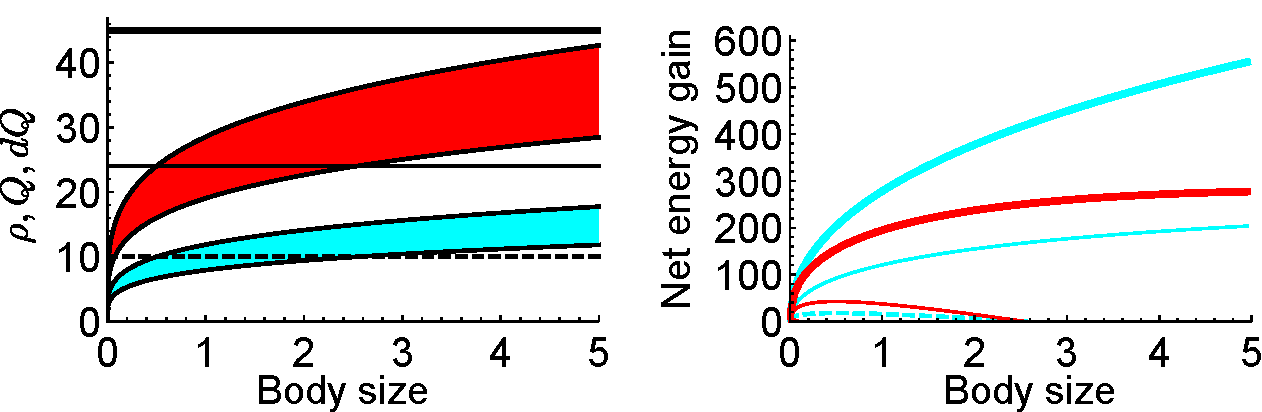
\includegraphics{appendix_fig}}
	\caption{Left panel illustrate the conditions in \cref{ineq:3} where $\rho$ needs to be within certain range.
	Cyan and red colors represents two environmental temperatures $T_e = 15, 25^\circ \rm{C}$, respectively.
  The upper bound of the shaded area ($Q$)is the right-hand side of \cref{ineq:3}.
  The lower bound of the shaded area ($dQ$)is the left-hand side of \cref{ineq:3}.
  The black horizontal lines represent $\rho = 10 \textnormal{ (dashed)}, 24 \textnormal{ (thin)}, 45 \textnormal{ (thick)}$.
  Right panel shows how net energy gain peaks at intermediate body size when $\rho$ is within a certain range based on the left panel.
  Remaining parameters: $\tau_f = 0.75, a_1 = 1., a_2 = 20 a_1, a_3 = 1, b_1 = b_2 = 0.75, a_3 = 0.5$.
	}
	\label{fig:ana}
\end{center}
\end{figure}

\bibliography{refs_energy_budget}
\end{document}
